% !TeX root = ../../main.tex
% Add the above to each chapter to make compiling the PDF easier in some editors.


\chapter{Results and Discussion}\label{chapter:results}

\section{Overview}
\section{Experiments Results}
\section{Benchmarking and Comparison}
\section{Concluding Remarks}


% \chapter{Framework, Setup and Implementation}\label{chapter:experiments2}
% Our aim is building a modular distributed deep reinforcement learning framework that is capable of running multiple environments \textit{(OpenAI Gym, DeepMind Control Suite, Unity Ml-Agents, Visdoom, Atari)} with the state of the art \textbf{(SOTA)} reinforcement learning algorithms in both single and multiple environments which supports single-node multi-cpu multi-gpu architecture.

% Our design features the reusability of modular components which are friendly coded in an efficient way with code decoupling and organized submodules.
% Along with easy customizable configurations for both agents and environments. Also using the visualization submodule to output training stats and performance with the help of tensorboard. Finally the ability to save and load pre-trained models for evaluating and testing the agents with option of rending the environment.

% \section{Architecture Overview}
% We architecture design has a modular interface that support custom networks, agents, and environments. 

% it provides multi-cpu and multi-gpu training along with parallel environments. 

% for debugging and evaluation we support tensorboard logging, model saving, reloading, evaluation, and rendering. 

% We also use \textit{tune} for hyperparameters tuning and optimization.

% The architecture is divided into multiple engines which support normal and distributed modes as describe here:

% \begin{figure}[!htb]%
%   \centering
%   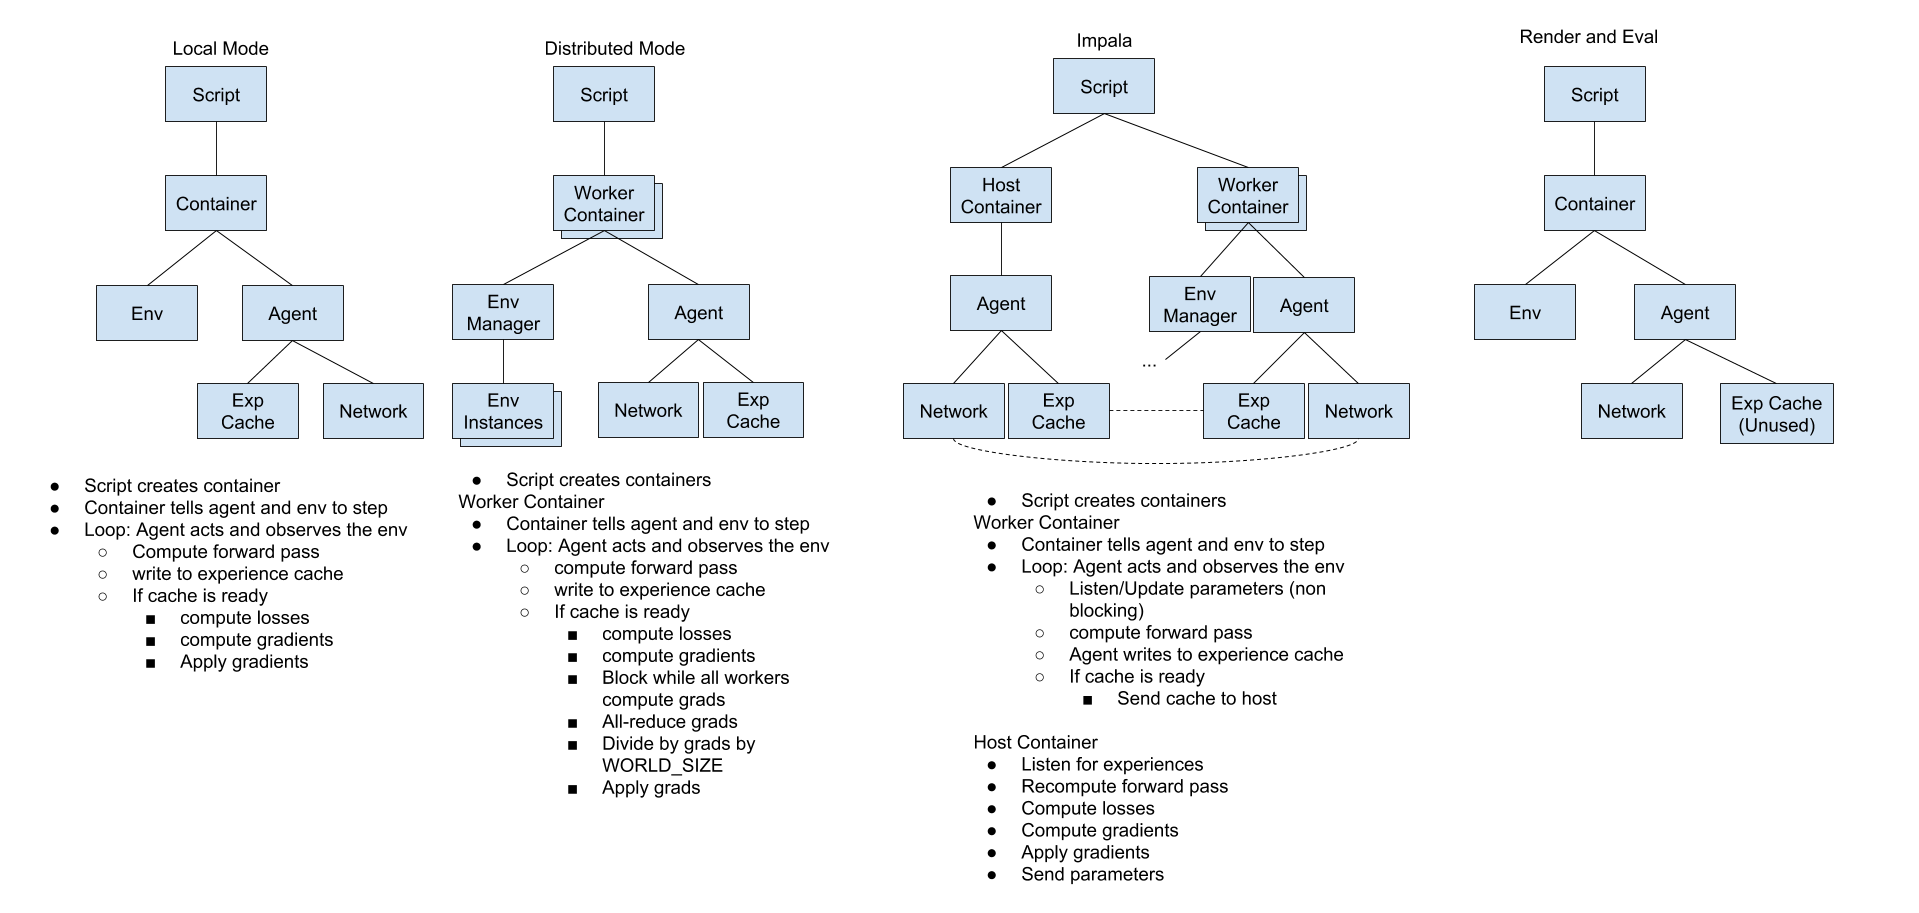
\includegraphics[width=\linewidth]{figures/architecture.png}%
%   \caption{Architecture Design}%
%   \label{fig:custom-reacher-xml}%
% \end{figure}

% \subsection{Engines}
% Engines contains the configurations for the experiments. it starts with initializing the environment manager and building the corresponding agent for the given environment, then it calls the container and start the training. 

% \subsection{Containers}
% Containers hold all of the application state. it's where the training process starts. Each subprocess gets a container in Towered and IMPALA modes.

% \subsection{Agents}
% An Agent acts on and observes the environment.With the state of the art algorithms and the support for multiple workers and distributed training

% \subsection{Networks}
% ModularNetwork classes. A ModularNetwork consists of a source nets, body, and heads. which is used to compute the actions for the given states of the environments.

% \subsection{Environments}
% Environments run in subprocesses and send their observation, rewards, terminals, and infos to the host process. They work pretty much the same way as OpenAI's code.



% % \section{Neurorobotics Platform Overview}

% \section{Our Experiment}
% Our experiment will be based on testing the performance among different environment and RL tools.

% \subsection{Overview} 

% The selected environment \textbf{(Reacher)} will be chosen as a task to be solved be different RL algorithms for continuous action space. This environment is available in both \textit{OpenAI Gym \& Unity ML-Agents} and we will implement similar environment for our Neurorobotics Platform to compare the result between the toolkits and see the results.

% \subsection{Description}
% In this environment, a double-jointed arm can move to target locations. A reward of +0.1 is provided for each step that the agent's hand is in the goal location. Thus, the goal of your agent is to maintain its position at the target location for as many time steps as possible.

% Additionally, Unity environment provides a version which contains 20 identical agents, each with its own copy of the environment. This environment is useful for distributed training as example of multi-agent environment which is useful for algorithms like \textbf{PPO, A3C, and D4PG} that use multiple (non-interacting, parallel) copies of the same agent to distribute the task of gathering experience.

% Illustration for the environments can be founded here:~\ref{fig:reacher-environment}


% % \begin{figure}%
% %     \centering
% %     \subfloat[OpenAI Gym]{{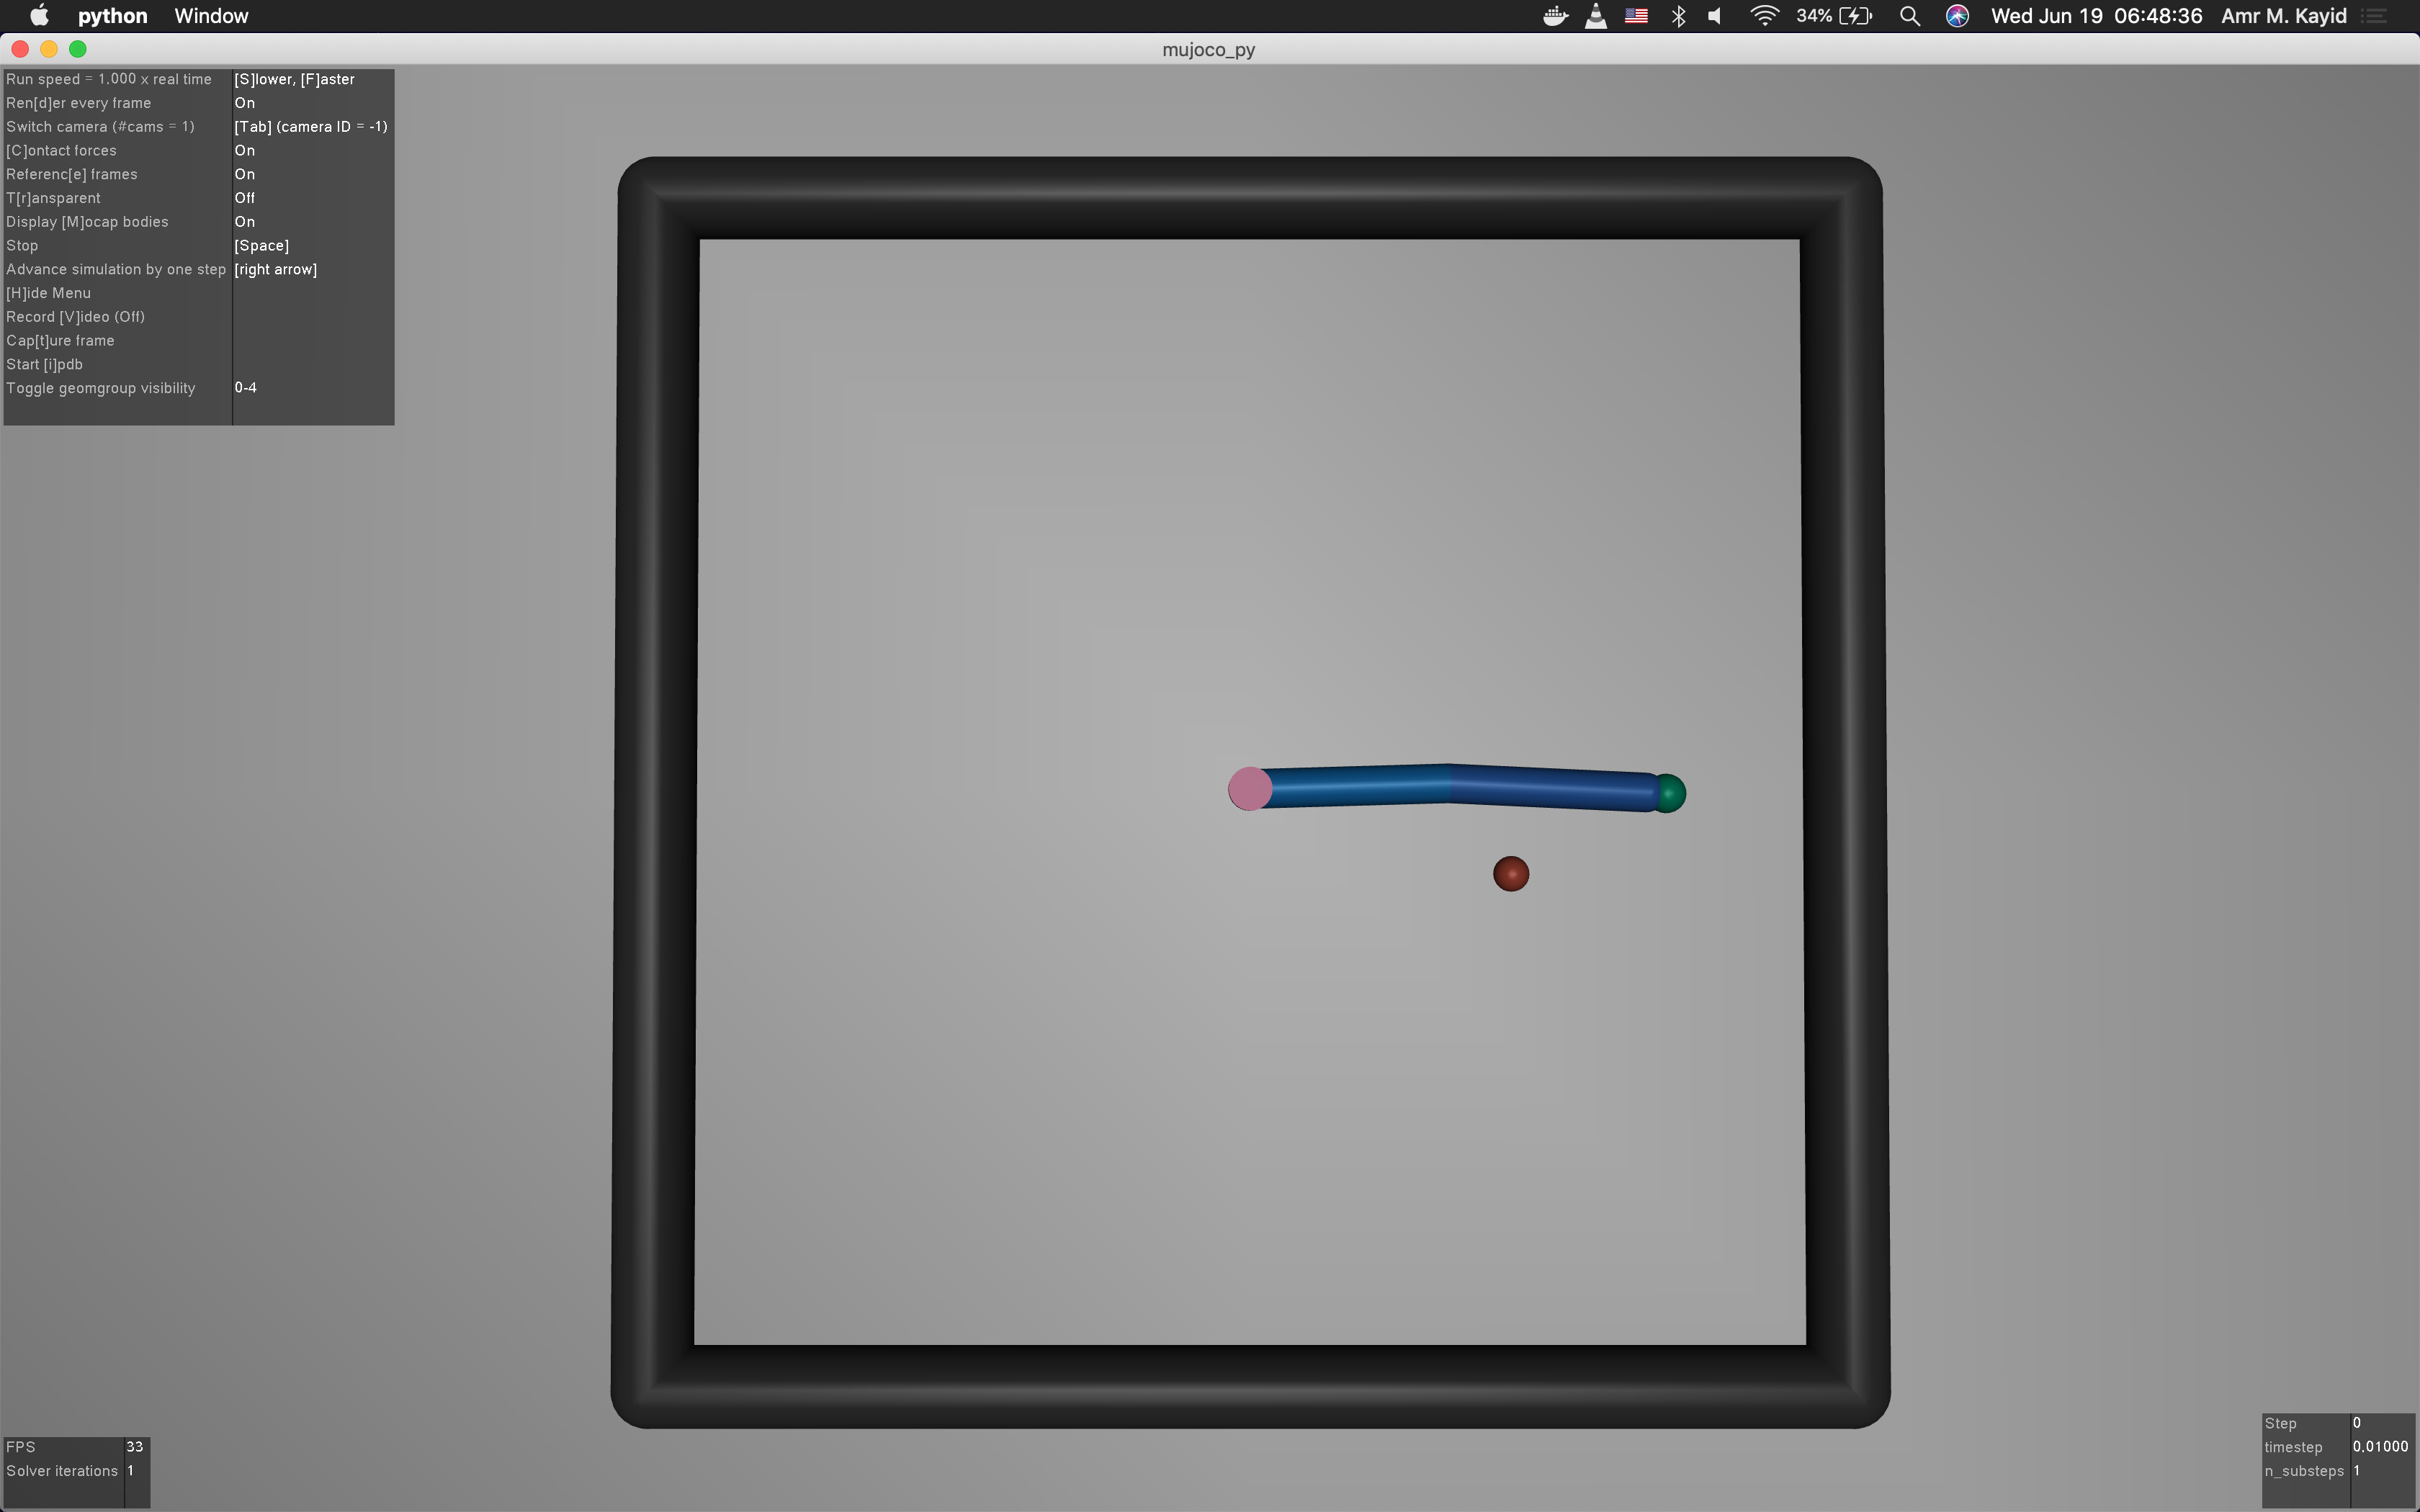
\includegraphics[width=7cm]{figures/envs/openai-gym-reacher-1.png} }}%
% %     \qquad
% %     \subfloat[Unity Single Agent]{{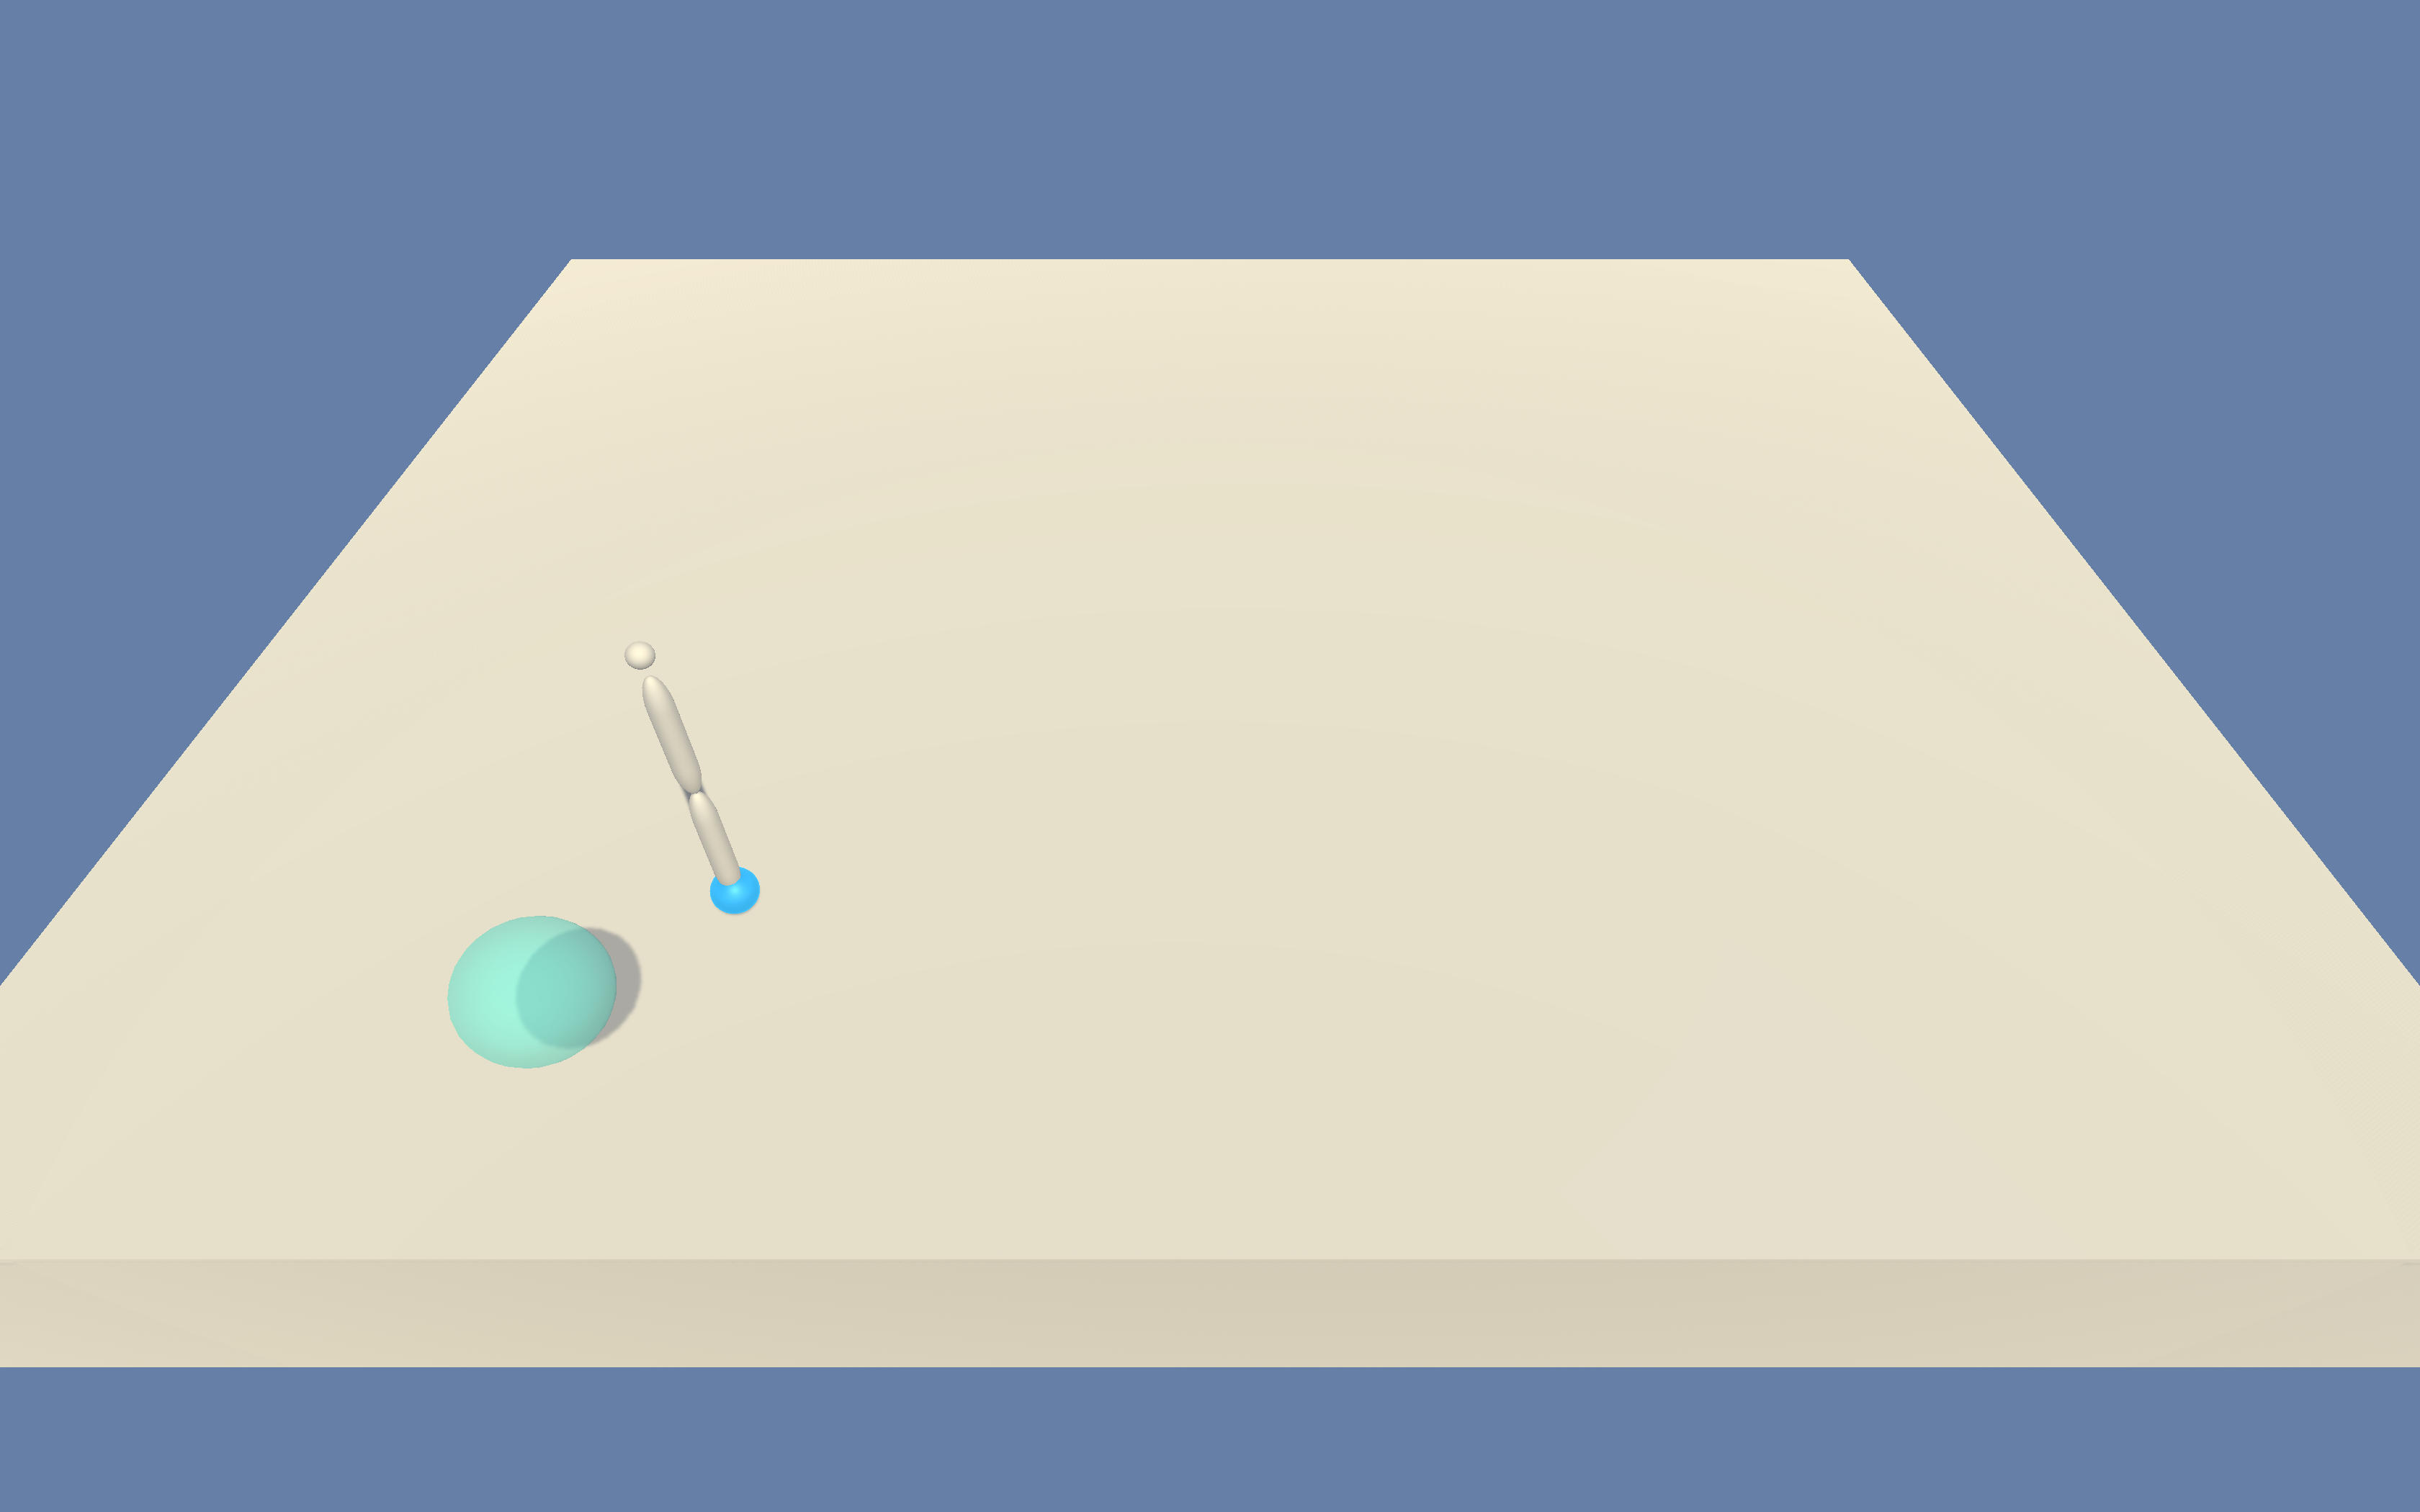
\includegraphics[width=7cm]{figures/envs/unity-reacher-1.png} }}%
% %     \subfloat[Unity Multiple Agent]{{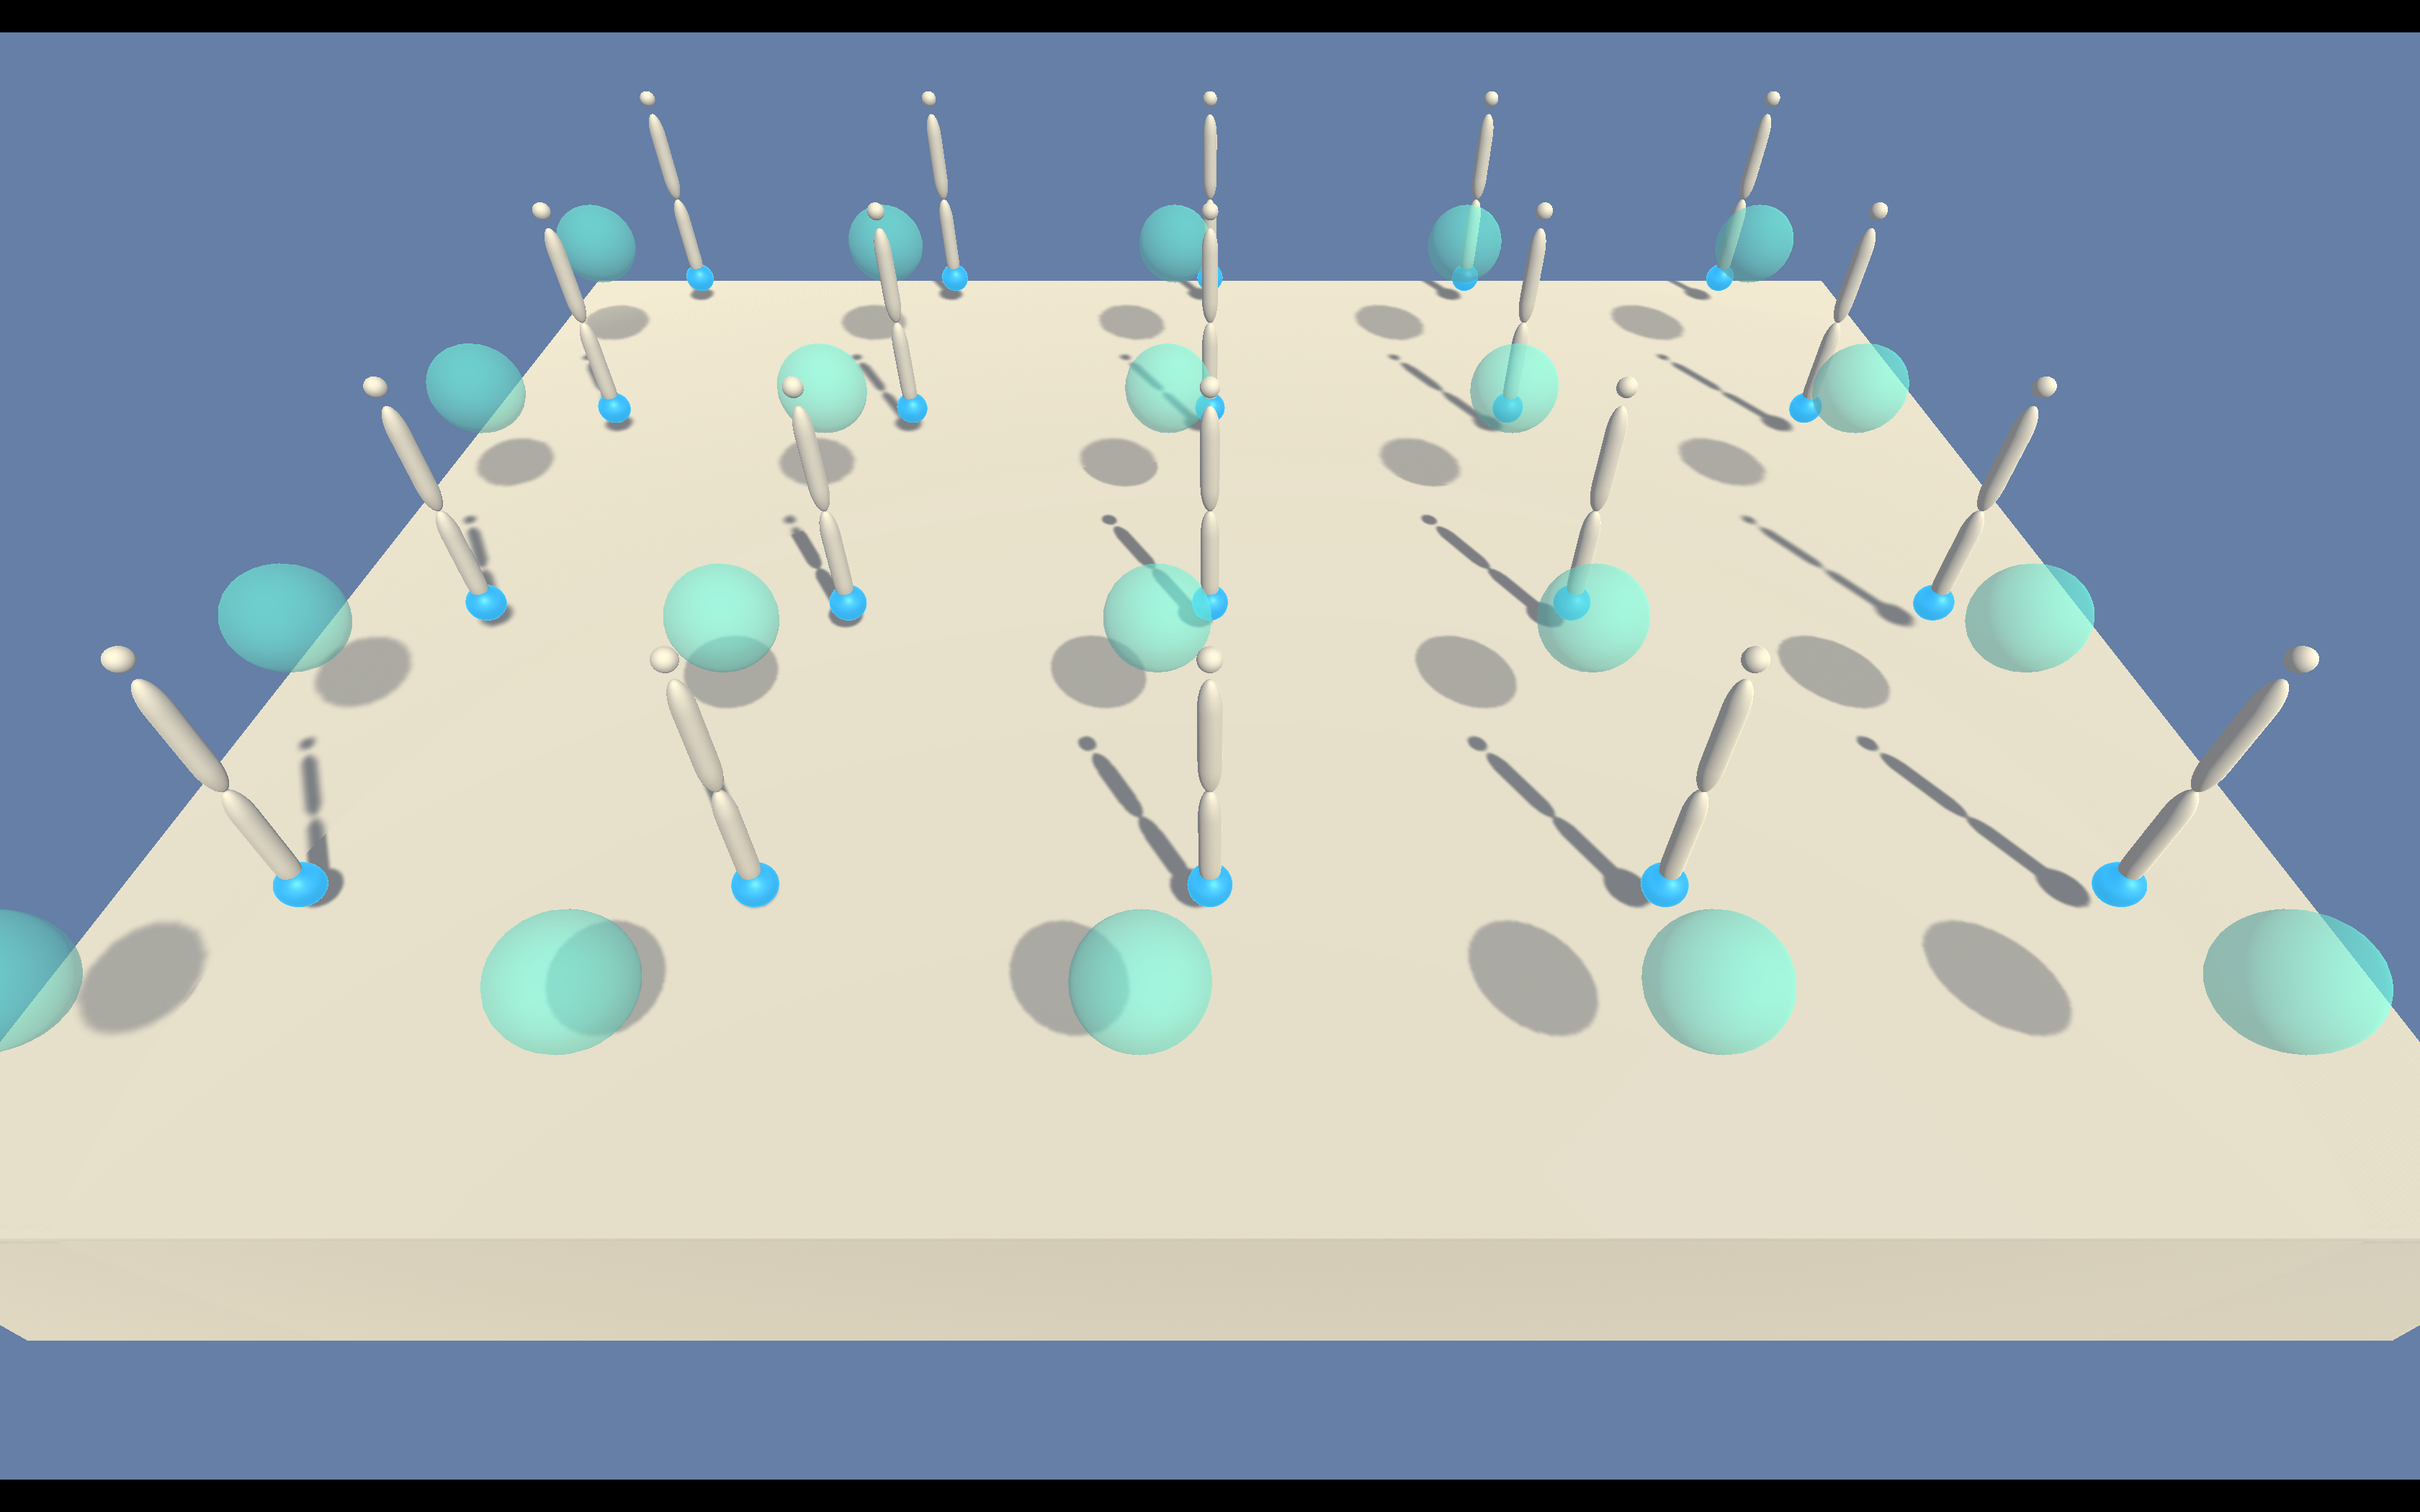
\includegraphics[width=7cm]{figures/envs/unity-reacher-20.png} }}%
% %     \caption{Reacher Environment}%
% %     \label{fig:reacher-environment}%
% % \end{figure}

% \clearpage

% \subsection{Environment custom xml model}
% The following figure~\ref{fig:custom-reacher-xml} is a model description of our custom environment in openai gym.

% \begin{figure}[!htb]%
%     \centering
%     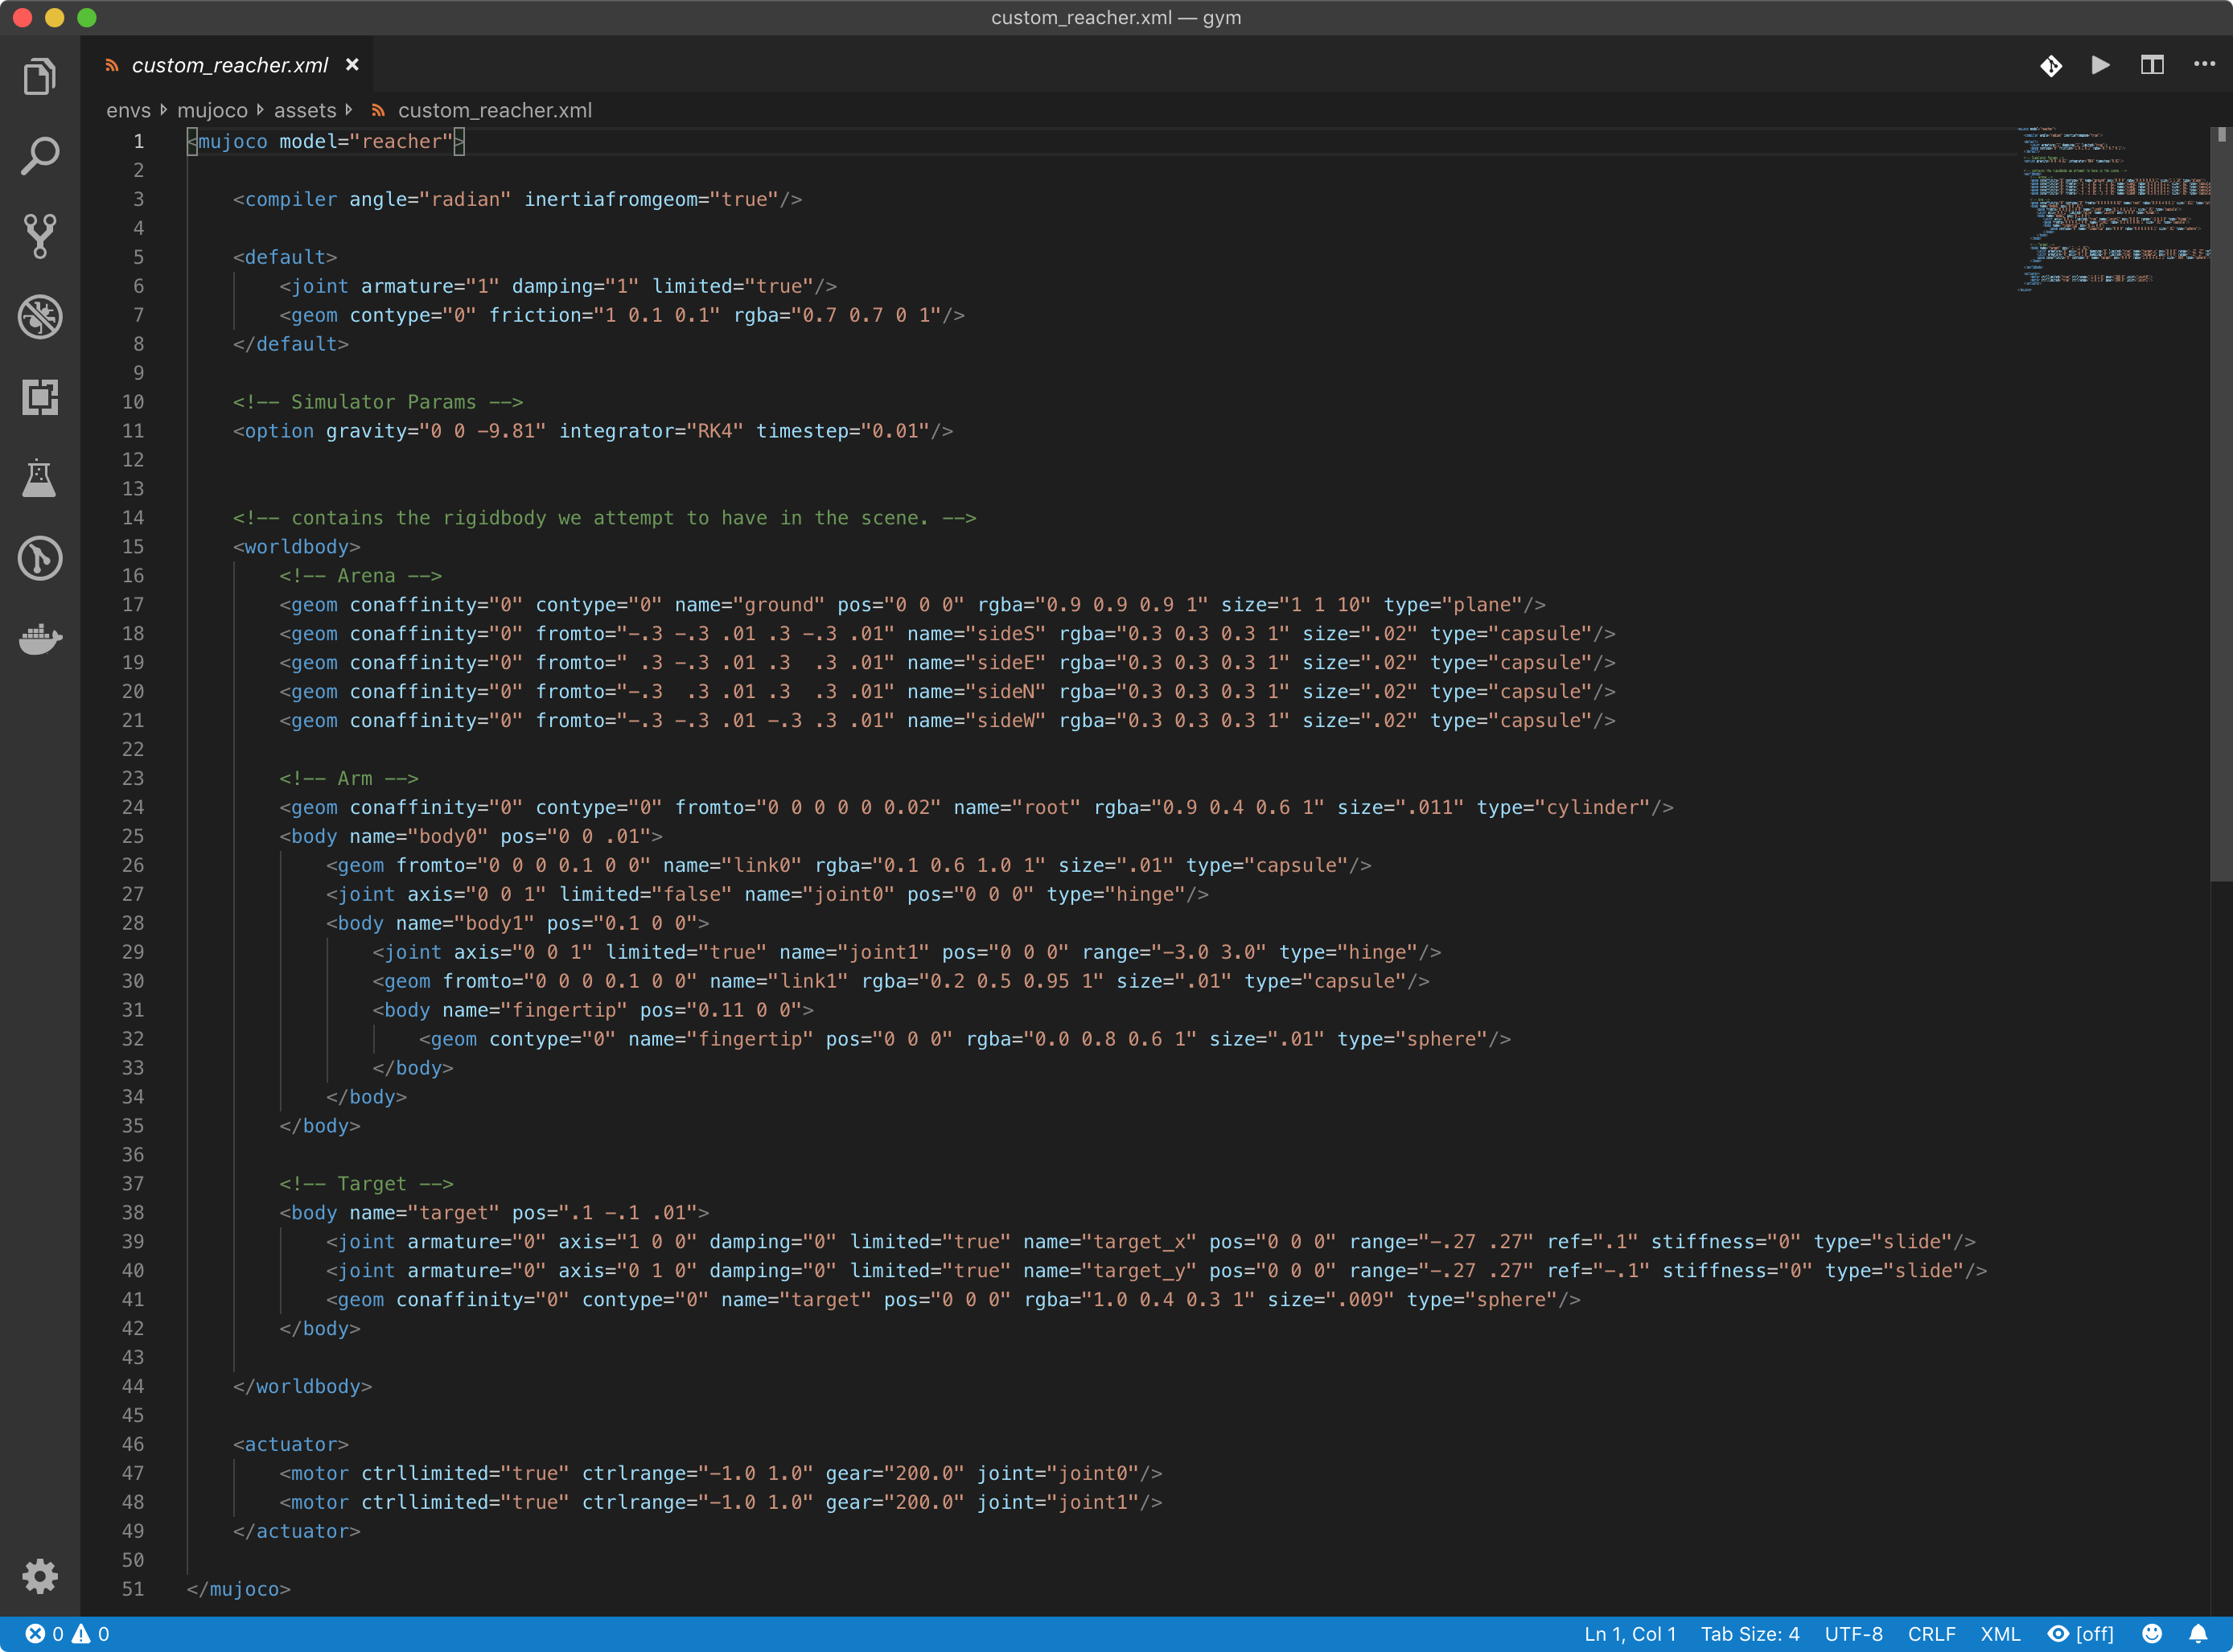
\includegraphics[width=\linewidth]{figures/envs/custom-reacher-xml.png}%
%     \caption{Custom reacher Environment}%
%     \label{fig:custom-reacher-xml}%
% \end{figure}

% The environment consists of a square scene that surround the double-linked robotics arm and a target goal location that gets generated randomly every episode.

% The double-linked robotics arm consist of two joints which can follow the target by moving in a range (-3.0, 3.0)
% The observation space consists of 

% \begin{table}[!htb]
%     \begin{center}
%       \begin{tabular}{l|c|r} % <-- Alignments: 1st column left, 2nd middle and 3rd right, with vertical lines in between
%         \textbf{Name} & \textbf{type} & \textbf{value}\\
%         \hline
%         Position and Rotation & float & self.sim.data.qpos.flat[2:]\\
%         Speed and Velocities & float & self.sim.data.qvel.flat[:2]\\
%         Distance between arm and target & float & self.get\_body\_com(``fingertip") $-$ self.get\_body\_com(``target")\\
%         Sine of position & float & np.sin(theta)\\
%         Cosine of position & float & np.cos(theta)\\
%       \end{tabular}
%       \caption{Observation Space}
%       \label{tab:table1}
%     \end{center}
%   \end{table}

% \subsection{agent actions}
% Each action is a vector with four numbers, corresponding to torque applicable to two joints. Every entry in the action vector should be a number between -1 and 1.

% \subsection{rewards}

% the reward function will be represented in A reward of \textbf{+0.1} is provided for each step that the agent's hand is in the goal location.
% Hence, the goal of the agent is to maintain its position at the target location for as many time steps as possible.

% Agents must get an average score of +30 (over 100 consecutive episodes, and over all agents). Specifically,
% The environment is considered solved, when the average (over 100 episodes) of those average scores is at least +30.
% % \clearpage

% \section{Methods}
% In order to solve this environment and also experiment the distributed algorithms and compare the results, we will be using the following algorithms:

% \begin{itemize}
%     \item Deep Deterministic Policy Gradient
%     \item A3C Algorithms
%     \item IMPALA
%     \item Ape-X 
% \end{itemize}

% We will start with VanillaPG as it's the simplest version of all the algorithms to test the behavior of the agent and the average reward gained. Followed by using A3C algorithm to test multiple workers and there effect on the agent policy. Then, we will apply threading and parallelization in both impala and ape-x along with the distributed experience replay for the environment states and compare the result with other algorithm and policies of the agent.

% \section{Software and Related Libraries}

% \begin{itemize}
%     \item OpenAI Gym
%     \item DeepMind Lab
%     \item Unity ML-Agents
%     \item Ray Project
% \end{itemize}

% \section{NRP Idea:}

% Since the nrp is a complete platform running on top of docker and it's reach frontend and experiment design can allow for rapid prototyping new environment,\\\\
% We can Create a custom reacher environment with multiple number of agents to distribute the learning process between them and make it multi-agent environment.
% This will allow us to reduce the latency and enhance the agents learning experience by communicating with each other directly in one experiment.

% % \begin{itemize}
% %     \item Transfer function is always running (10ms), the agent won't be able to learn as if the agent select an action it will be executed each 10ms without waiting to observe the new state.
% %     \item Can we randomly render objects or create it using python code?
% %     \item Can we destroy the generated objects?
% %     \item environment modeling and rendering with the step function (huge)
% %     \item scaling problem? we won't be able to run multiple workers using the nrp experiment environment
% %     \item compatibility, old python version, jupyter notebook
% % \end{itemize}


% % \section{The Implementation}
